\section{Web Drawing Prototype}
\label{prototype:WebDrawing}
For this prototype I wanted to explore the feasibility of drawn text within a webpage, crucially I needed to ensure that this would work on an iPad with Apple Pencil as this is my main note taking device.

\begin{figure}[H]
    \centering
    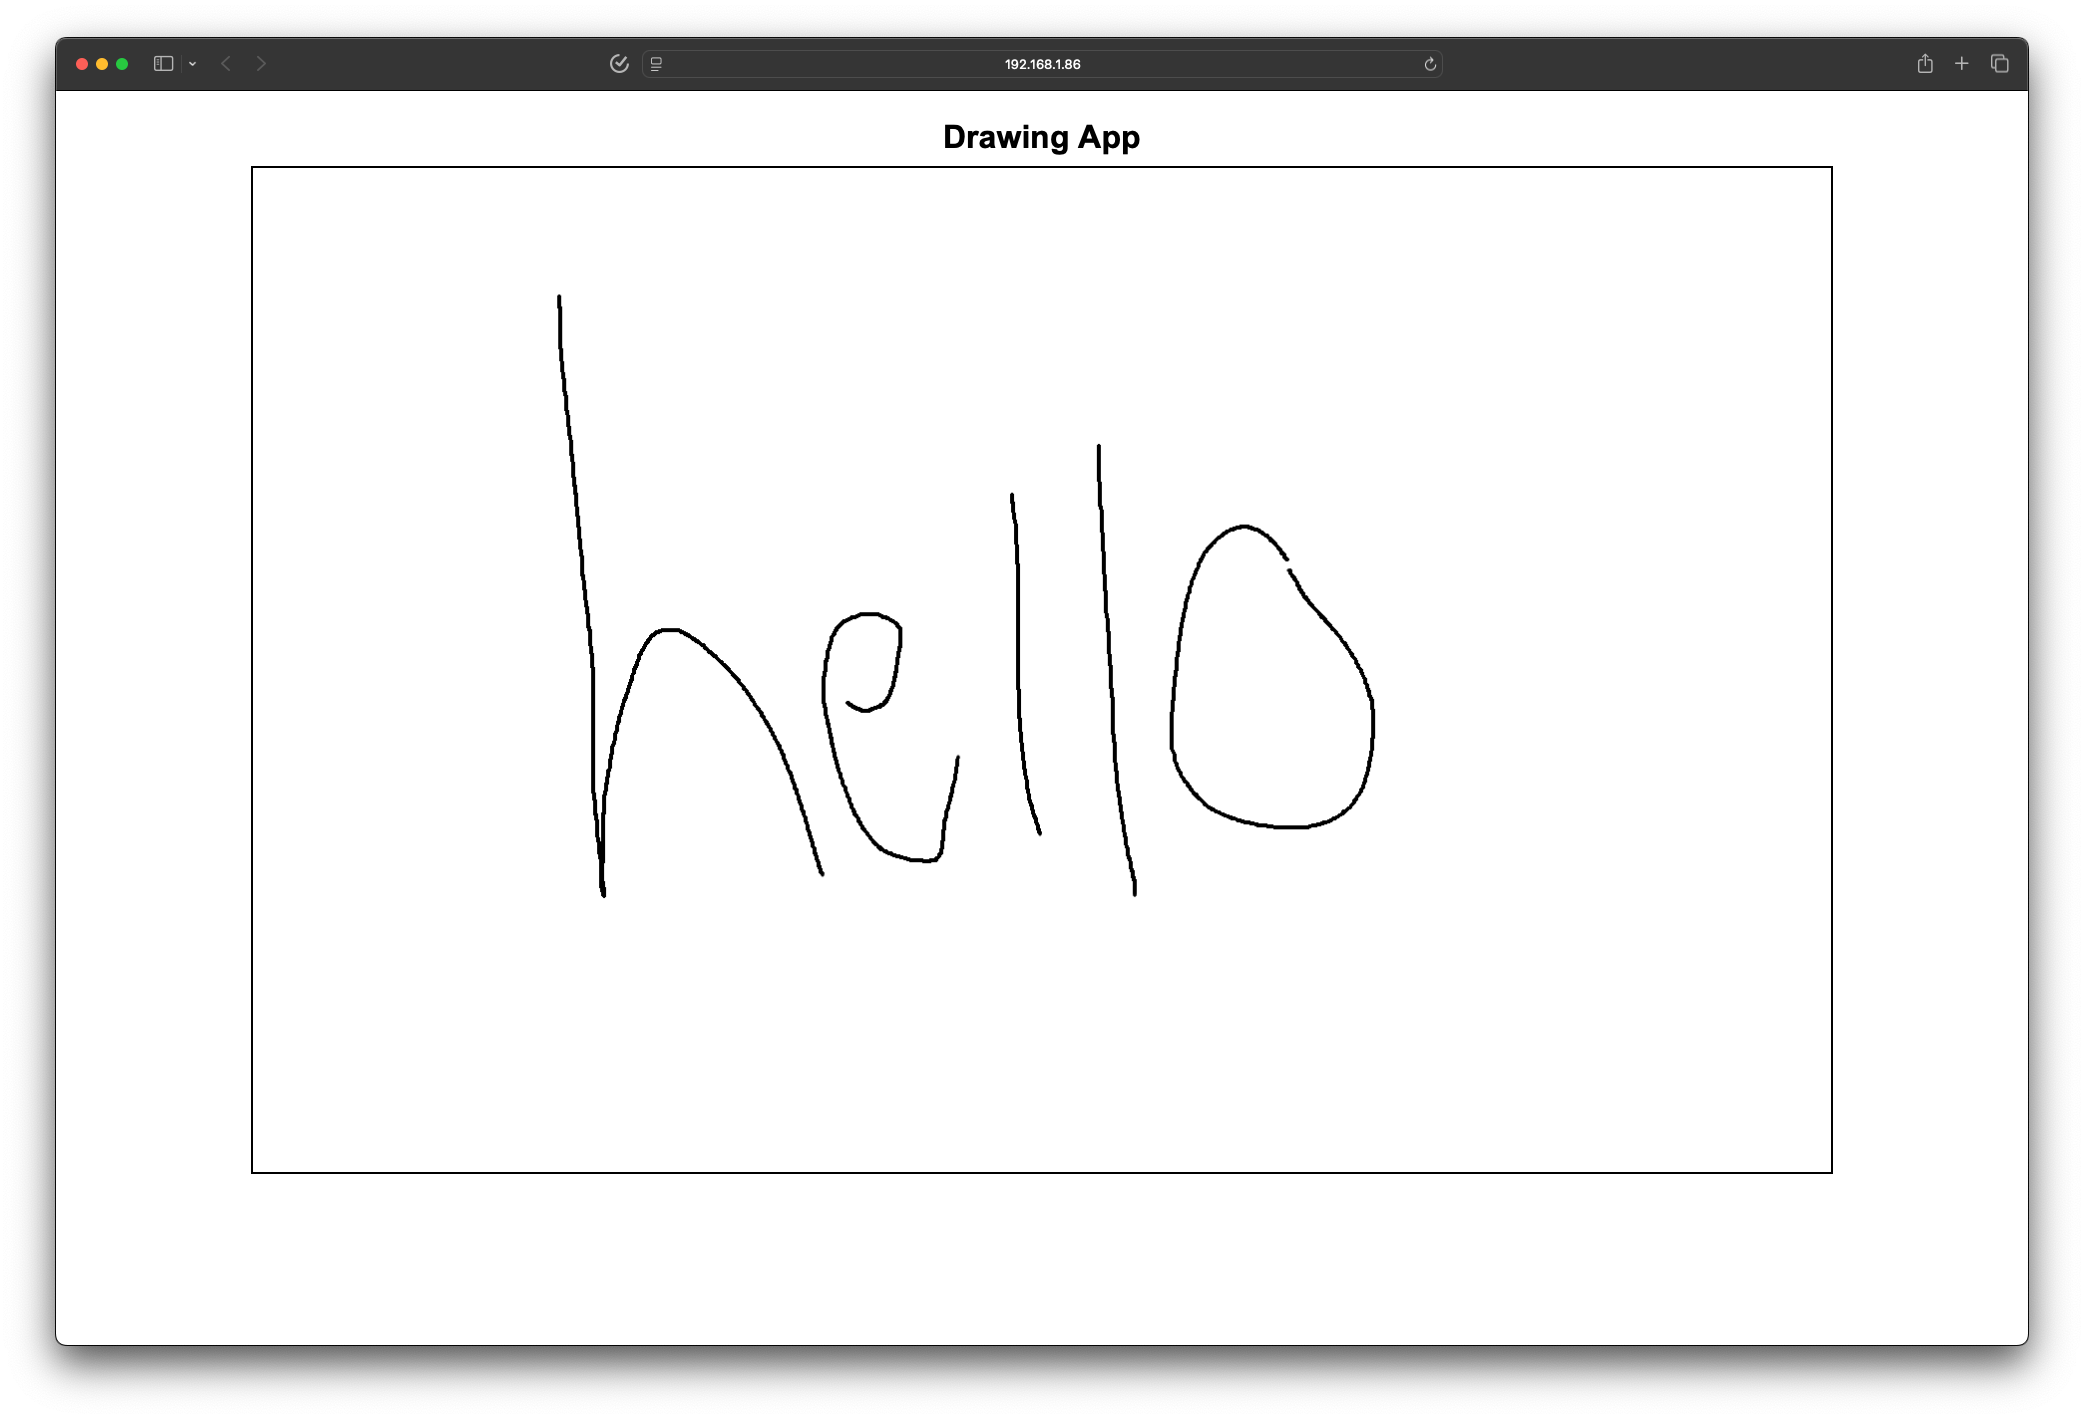
\includegraphics[width=0.8\textwidth]{Prototype/7_WebDrawing/media/MacbookSS.png}
    \caption{Writing with my macbook trackpad}
    \label{fig:WebDrawingPrototype1}
\end{figure}

\begin{figure}[H]
    \centering
    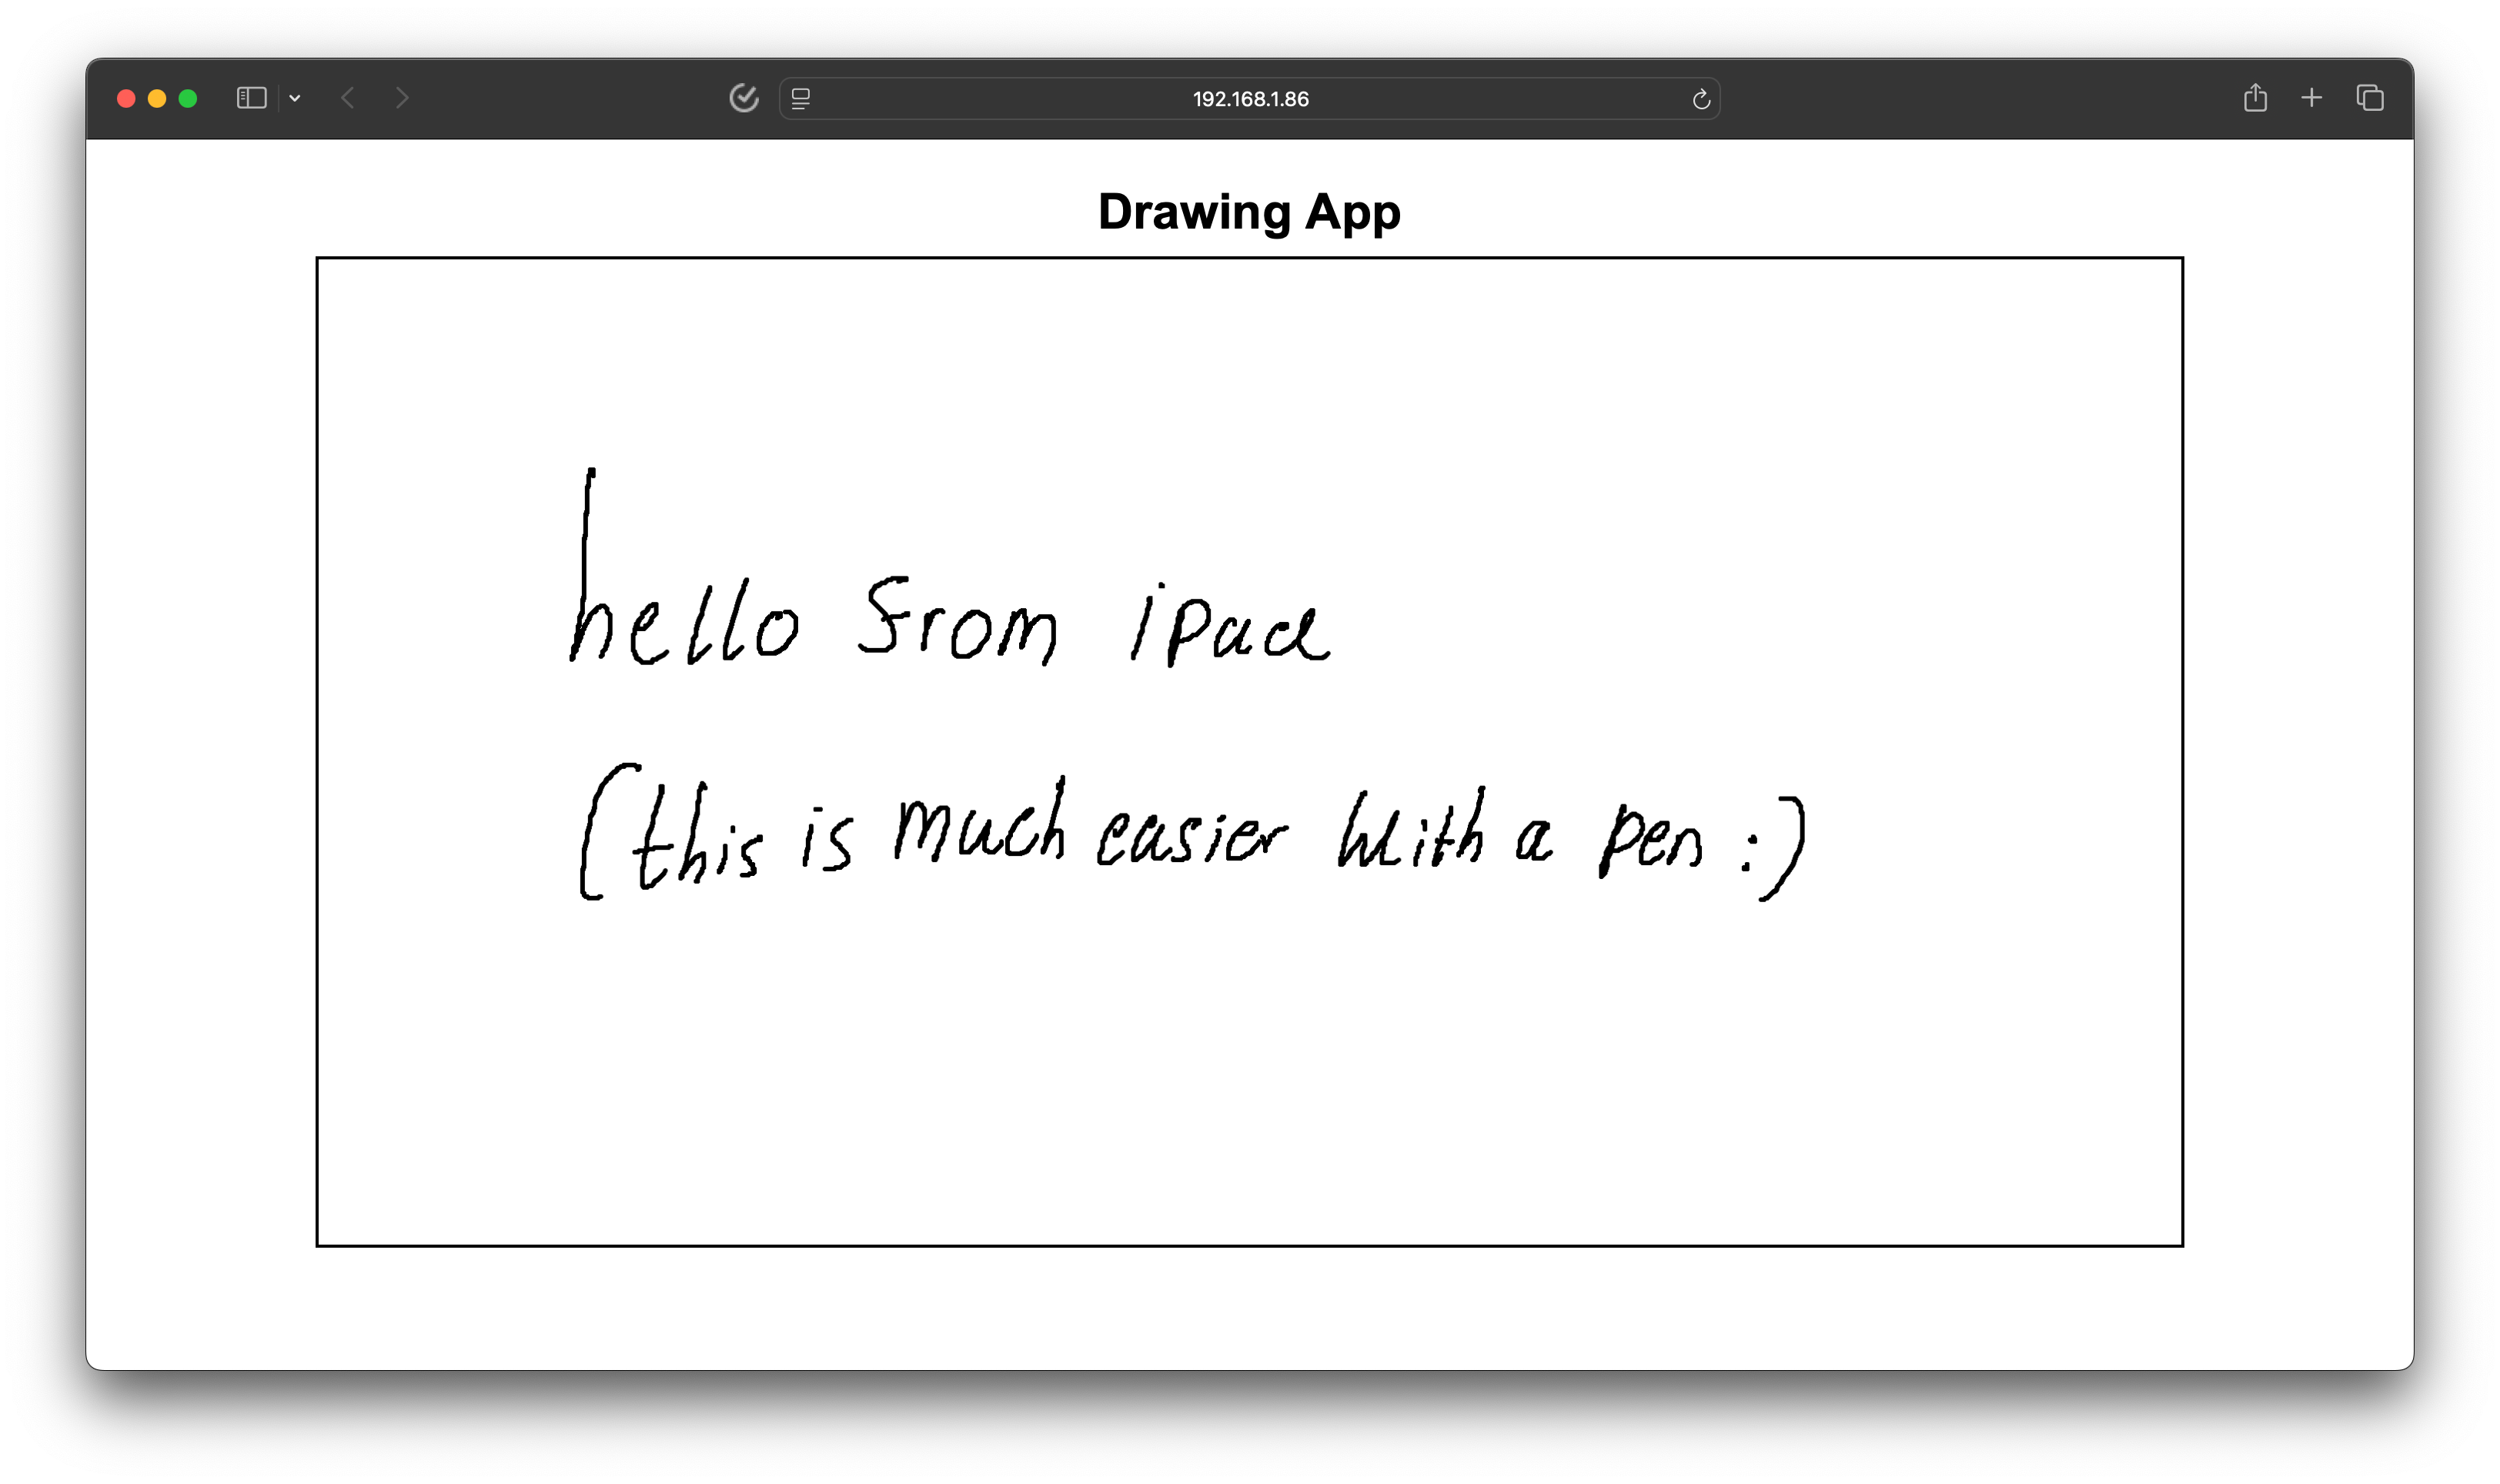
\includegraphics[width=0.8\textwidth]{Prototype/7_WebDrawing/media/IpadSS.png}
    \caption{Writing with my ipad + Apple Pencil}
    \label{fig:WebDrawingPrototype2}
\end{figure}
\subsection*{Python Code}

This server code is relatively similar to the previous prototype, it allows multiple users to connect and send messages in real-time, but this time it also supports drawing on a canvas.

\inputminted[linenos, tabsize=1, breaklines]{python}{Prototype/7_WebDrawing/media/PythonCode.py}

\subsection*{HTML Code}

This code runs on the clients device in the browser and connects to the Python server, allowing users to draw on a canvas.

\inputminted[linenos, tabsize=1, breaklines]{html}{Prototype/7_WebDrawing/media/HtmlCode.html}

